\documentclass{article}
\usepackage{textcomp}
\usepackage[english]{babel}
\usepackage[utf8]{inputenc}
\usepackage{lmodern}
\usepackage{textcomp}
\usepackage[T1]{fontenc}
\usepackage{ucs}
\usepackage{amssymb}
\usepackage{amsmath}
\usepackage{courier}
\usepackage{graphicx}
\usepackage{a4wide}

\newcommand{\quality}[1]{q_{#1}}
\newcommand{\minfun}{\text{min}}
\newcommand{\realvec}[1]{\mathbf{#1}}
\newcommand{\norm}[1]{\left\| #1 \right\|}
\newcommand{\derivative}[2]{\frac{\partial #1}{\partial #2}}
\newcommand{\timederivative}[1]{\derivative{#1}{t}}
\newcommand{\realnumber}{\mathbb{R}}
\setcounter{secnumdepth}{2}




% Style used for devices.
\newcommand{\device}[1]{\texttt{#1}}

% Words to denote the devices that we are talking about
\newcommand{\anemobox}{\device{anemobox}}
\newcommand{\phone}{\device{phone}}
\newcommand{\anemolab}{\texttt{anemolab}}

% Abbreviations for the above words
\newcommand{\abbrbox}{\device{[B]}}
\newcommand{\abbrphone}{\device{[P]}}
\newcommand{\abbrlab}{\device{[L]}}


\author{Jonas Östlund\\jonas@anemomind.com}
\date{\today}
\title{Anemomind Nividic Data Transfer Architecture}

\begin{document}
\maketitle
\section{Introduction}
The purpose of this document is to outline the architecture for transferring data between the different devices involved with the Nividic product. Specifically, there are three types of devices: an \anemobox{}, a mobile \phone{} or tablet, and \anemolab{}. We also outline a high-level description of the protocol used to communicate between the devices.

\section{Requirements}
The architecture should at least accomodate the following operations that will be necessary for Nividic:
\begin{itemize}
  \item Move log files from \anemobox{} to \anemolab{}
  \item Move photos and notes from \phone{} to \anemolab{}
  \item Move calibration parameters from \anemolab{} to \anemobox{}
\end{itemize}
but should be general enough to allow for other type of data transfer too in later product releases.

Different architectures and protocols are defined for different requirements, constraints and use cases. For instance, the TCP/IP suite is designed for robust delivery of data over the internet, whereas the UDP protocol is designed for low latency. The architecture and high-level outline of the protocol in this document is designed according to the following assumptions and considerations:
\begin{itemize}
  \item \textbf{Storage capacity} on any device \textbf{is abundant}. For instance, there are Micro SD cards that can store thousands of photos or several weeks of boat logs. Such cards can be on both the \anemobox{} and \phone{}. Cloud storage for \anemolab{} is also abundant. Therefore, we assume that there is no need to delete data prematurely, before we are absolutely sure that it has reached its destination.
  \item \textbf{Communication links} between two devices \textbf{rarely exist}. For instance, a sailor may be sailing mostly in his week-end but spend the rest of the week working. Therefore, there will only be a communication link (e.g. bluetooth) between his mobile phone and the boat in the week-end when he is sailing, but not when he is away from his boat with the phone in his pocket. Likewise, it may not be possible to always establish a communication link between the mobile phone and the internet if he is sailing far away from the coast or along the coast of a foreign country where data traffic is limited. 
  \item \textbf{Robustness over latency.} The information that is transferred between devices can be very valuable, not the least in terms of time and effort. For instance, a log file containing hours of recorded data correspond to the same amount of time of real sailing, maybe in tough and cold conditions. Such recordings must not be lost when they are transferred. It is usually more important that the transfer is robust than slightly reducing the time the user has to wait for some operation. We thus adopt a policy of eagerly trying to propagate data from one device to another device in order to maximize the chance that the data will eventually reach its destination.
\end{itemize}

For the Nividic release, we assume that there will be communication links between \anemobox{} and \phone{} (such as bluetooth), and between \phone{} and \anemolab{} (e.g. with TCP/IP), as illustrated in Fig.~\ref{fig:arch}.
\begin{figure}
\begin{tabular}{cc}
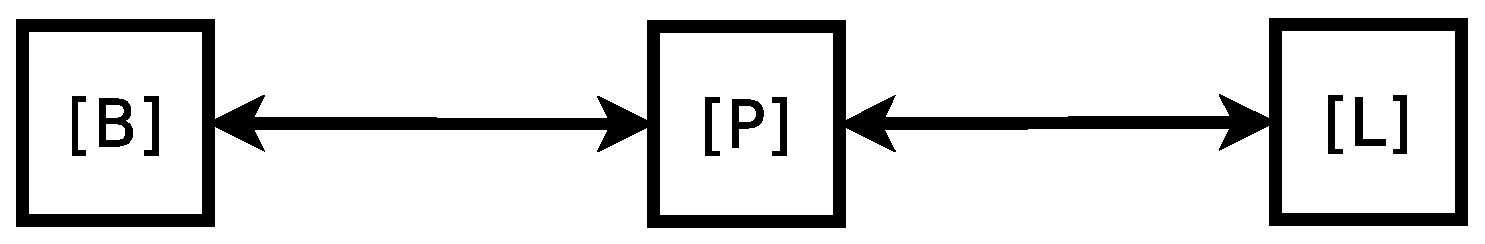
\includegraphics[width=0.48\textwidth]{archnividic.eps} & 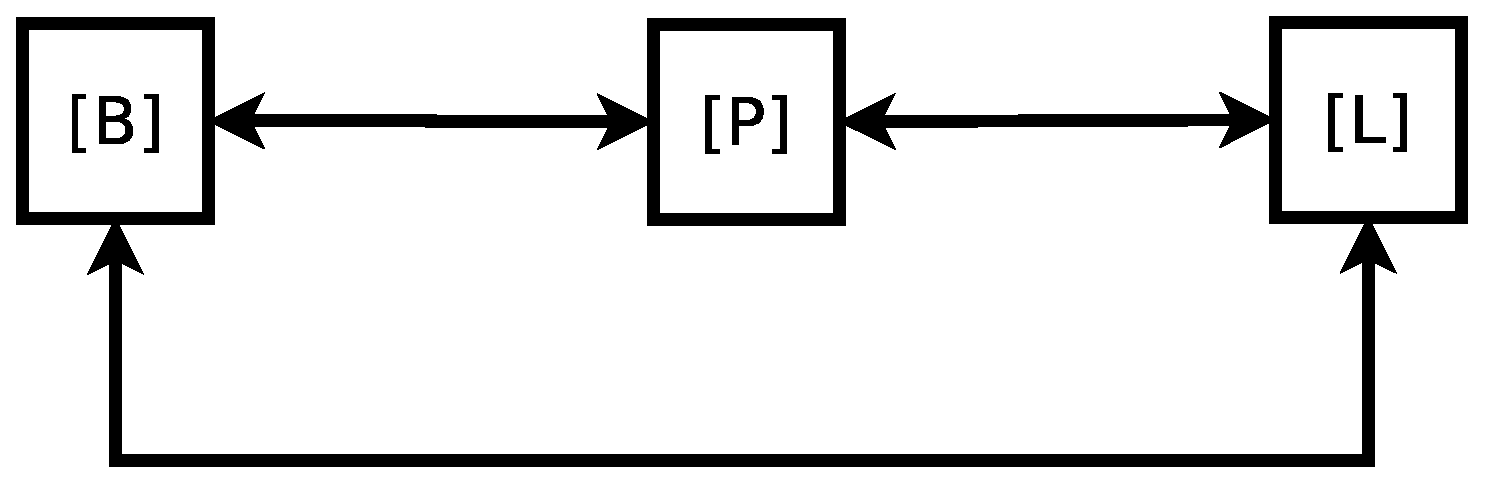
\includegraphics[width=0.48\textwidth]{archlater.eps} \\
(a) & (b)
\end{tabular}
\caption{Communication architectures, where \abbrbox{} is the \anemobox{}, \abbrphone{} is the \phone{} and \abbrlab{} is \anemolab{}. For the Nividic release (a) we assume that there is no communication link between the anemobox \abbrbox{} and the server \abbrlab{}. For later releases (b), we can imagine that such a link exists and our architecture and protocols should allow for that.}
\label{fig:arch}
\end{figure}

In order to better understand the requirements that drive the specification of the architecture and protocol, we will consider two use cases. The first use case outlines the easy case where the anemobox can talk more or less directly with the web server via the phone. The second use case is more difficult in the sense that two communication links are not available at the same time.

\subsection{Use case I: Continuous communication links}
\label{sec:easycase}
In this scenario, a sailor is on the sea with his sailboat, of the type Surprise. He has brought his mobile phone with him and the anemobox is installed on his boat. He is also sailing close to the coast and has a good internet connection to his phone. He is recording boat logs. These boat logs are continuously transferred from the anemobox to the mobile phone, and then transferred from the mobile phone to the server. After a few hours of sailing, he wants to update the calibration of his instrument, so he presses a button on his mobile phone to start calibration and a few minutes later, the calibration is done and transferred from the server to the anemobox. For the last quarter of an hour, there has been another Surprise in front of him. Thanks to a more accurate calibration, he is able to pass it eventually.

\subsection{Use case II: Discontinuous communication links}
\label{sec:hardcase}
In this scenario, a sailor is on the sea with his sailboat, sailing for a week-end. He has a mobile phone with him that is talking over bluetooth to the anemobox onboard. However, this sailor is a more modest man and he only has a prepaid phone with limited data traffic, so his phone rarely has an internet connection except when is at home connected to the WLAN. He records data on the anemobox that are transferred to the memory of the phone and saved there. When he comes home on the Sunday evening, he connects his phone to the WLAN and boat logs are uploaded to the server. Fresh calibration parameters are calculated and sent back from the server to the phone. The next week-end when he goes sailing, those parameters are transferred from the phone to the anemobox on his boat.

\section{Mailbox Model}
The mailbox model can be used to design a system that will work for either one of the two use cases in the previous section. In this model, every device has a target mailbox in its memory. It also has a temporary mailbox on some of the other devices. For instance, the server will have a target mailbox in its memory and a temporary mailbox on the phone and a temporary mailbox on the anemobox. Likewise, the phone will have a target mailbox in its memory and a temporary mailbox on the anemobox and a temporary mailbox on the server. The anemobox will also have a target mailbox in its memory and a temporary mailbox on the phone and one on the server. This is illustrated in Fig.~\ref{fig:mailboxes}.
\begin{figure}
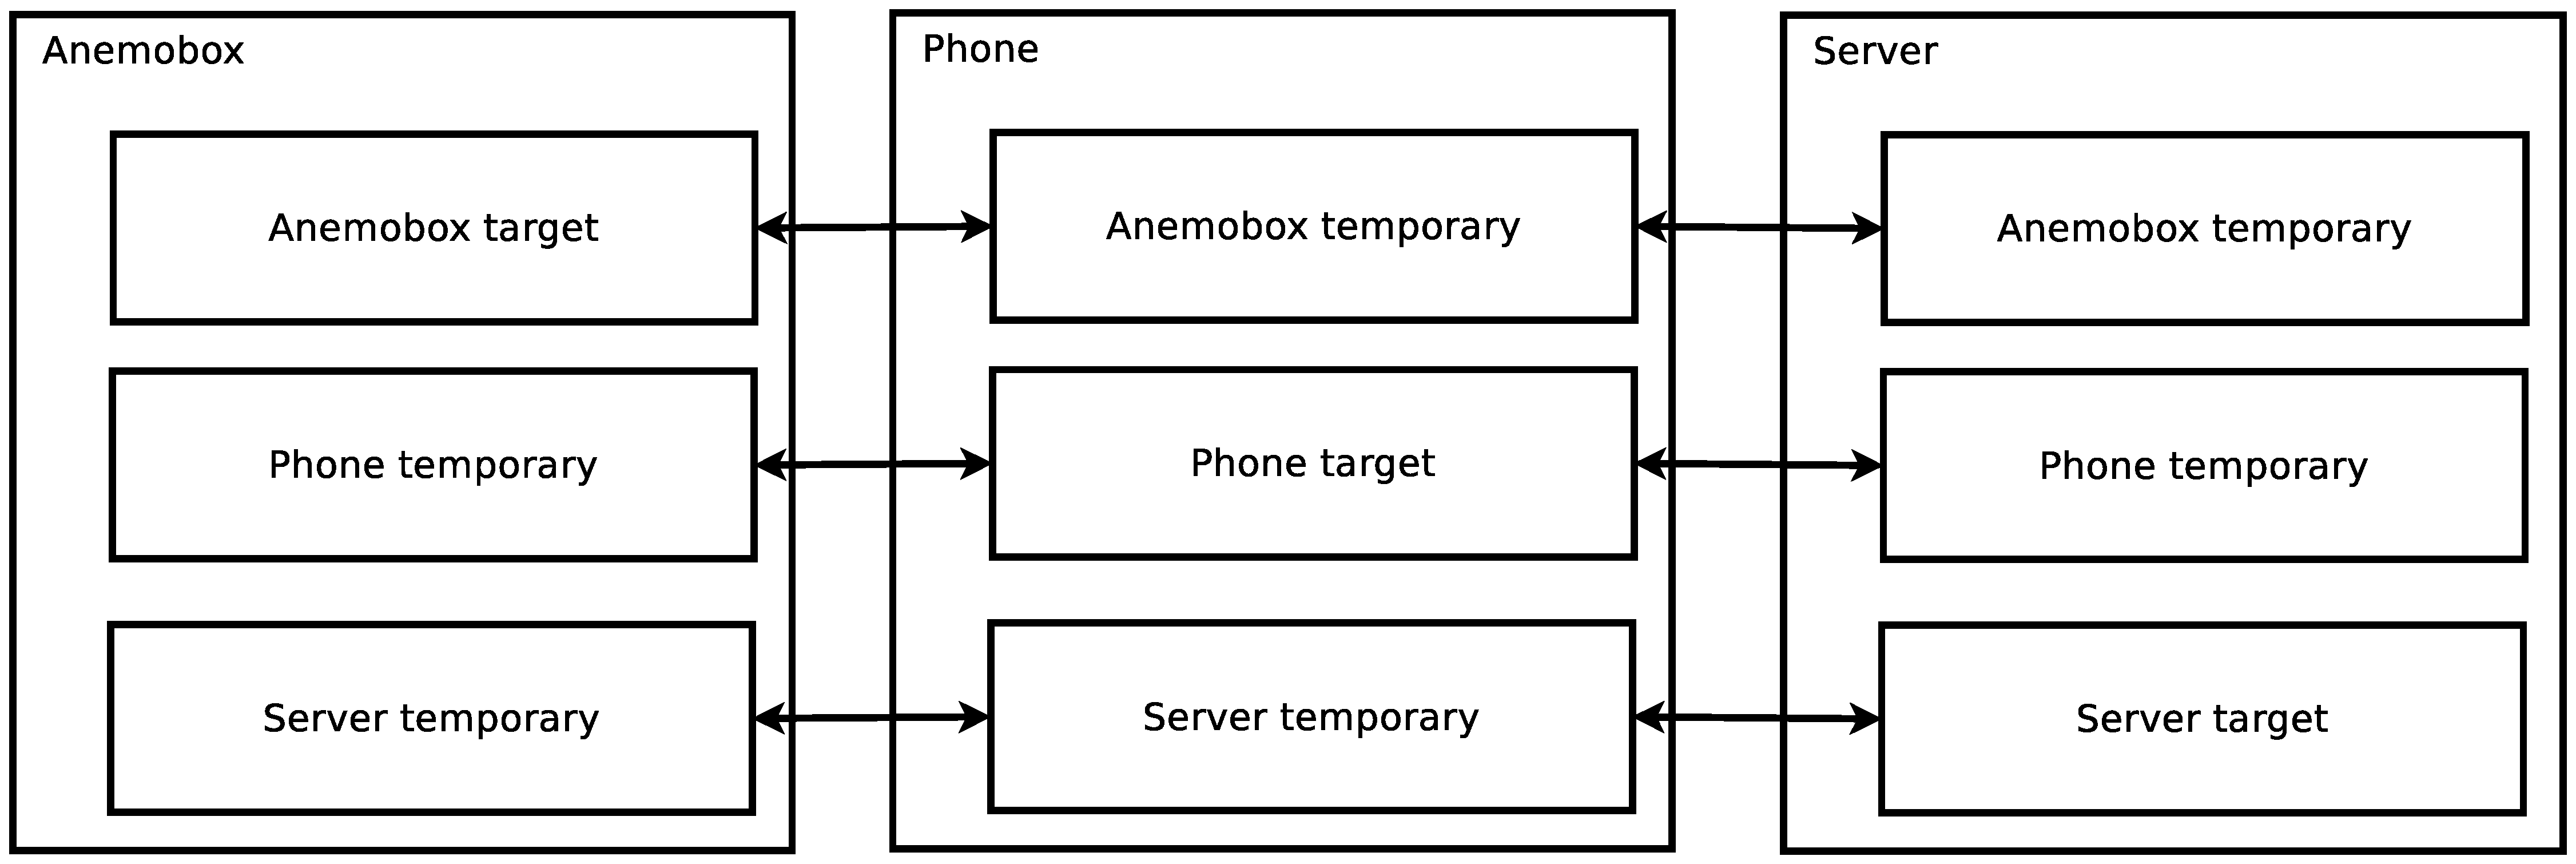
\includegraphics[width=\textwidth]{mailboxes.eps}
\caption{Mailbox model. Double-directed arrows are drawn between mailboxes that can synchronize in the Nividic version.}
\label{fig:mailboxes}
\end{figure}
We assume that we apply this model for a particular boat. Since Nividic will be used with several boats, there will be one mailbox for every boat on the server. On the other devices, however, there will rarely be mailboxes related to more than one boat.

Transferring a piece of data, that we will refer to as a \textbf{packet}, is done by synchronizing pairs of mailboxes until the packet reaches its destination. Multiple versions of the same packet can live on different devices simultaneously.

\subsection{Packet format}
A packet is a data structure with the following fields:

\begin{tabular}{l p{30em}}
  \texttt{from} & The identity of the sender. \\
  \texttt{to} & The identity of the receiver. \\
  \texttt{status} & A code that determines the status of the packet. Can be \texttt{in-progress} or \texttt{delivered}. \\
  \texttt{packet-id} & A code that uniquely identifies the packet. \\
  \texttt{label} & A code that specifies what kind of contents the packet contains.\\
  \texttt{data} & The data to be delivered.
\end{tabular}

Some explanations may be useful. The codes in the \texttt{from} and \texttt{to} fields must uniquely identify the device (\anemobox{}, \phone{} or \anemolab{}) and the boat identity related to a mailbox. The status code indicates where the packet is in the life cycle. In the beginning of the life cycle when the packet is created, its status is \texttt{in-progress}. Once it has been delivered, the packet is replaced by a similar packet where the status has been changed to \texttt{delivered}. A \texttt{packet-id} uniquely identifies the packet and is computed from the identity of the sender, the current time and a counter variable on the sender. The \texttt{label} specifies what type of packet it is used by a higher level protocol than defined in this document. It can be anything except for \texttt{collect-garbage} that we will explain in section \ref{sec:gc}. The \texttt{data} fields is the actual data to be carried. Its format is defined by a protocol and it should be clear by the \texttt{label} what the format is.

\subsection{Sending a packet}
When a packet is to be sent all the fields are filled in with information. In particular, the \texttt{status} field is set to \texttt{in-progress} and the \texttt{data} field is filled with the data to be sent. The packet is put in a temporary mailbox belonging to the target mailbox, on the sending device. Whenever that mailbox is synchronized with a corresponding mailbox on some other device, the packet is updated as explained in section~\ref{sec:sync}.

\subsection{Pairwise synchronization}
\label{sec:sync}
Delivering a packet from one device to another device can be broken down to a set of pairwise synchronizations of mailboxes. When a pair of devices are connected and synchronize, every pair of corresponding mailboxes that exist on both devices are synchronized. When two mailboxes are synchronized, all packets that exist on one or both of the mailboxes are considered. How two mailboxes are synchronized for a particular packet can be explained by a few simple rules.
\begin{itemize}
  \item When the packet only exists on one of the two devices, an identical copy of the packet is put on the other device, Fig.~\ref{fig:rules}(a, b). If the packet has the status code \texttt{in-progress}, putting the packet on the other mailbox means that the packet and the data that it carries propagates towards the destination, (a). If the packet has the status code \texttt{delivered}, putting the packet in the other mailbox means that the information that the packet has been sent is being propagated back to the sender, (b).
  \item When the packet exists on both devices having the status of \texttt{in-progress} on one device and the status of \texttt{delivered} on the other device, the packet with status \texttt{in-progress} will have its status updated to \texttt{delivered} and its data will be removed so that the package takes up less space on the device, Fig.~\ref{fig:rules}(c).
\end{itemize}

\begin{figure}
  \begin{tabular}{ccc}
    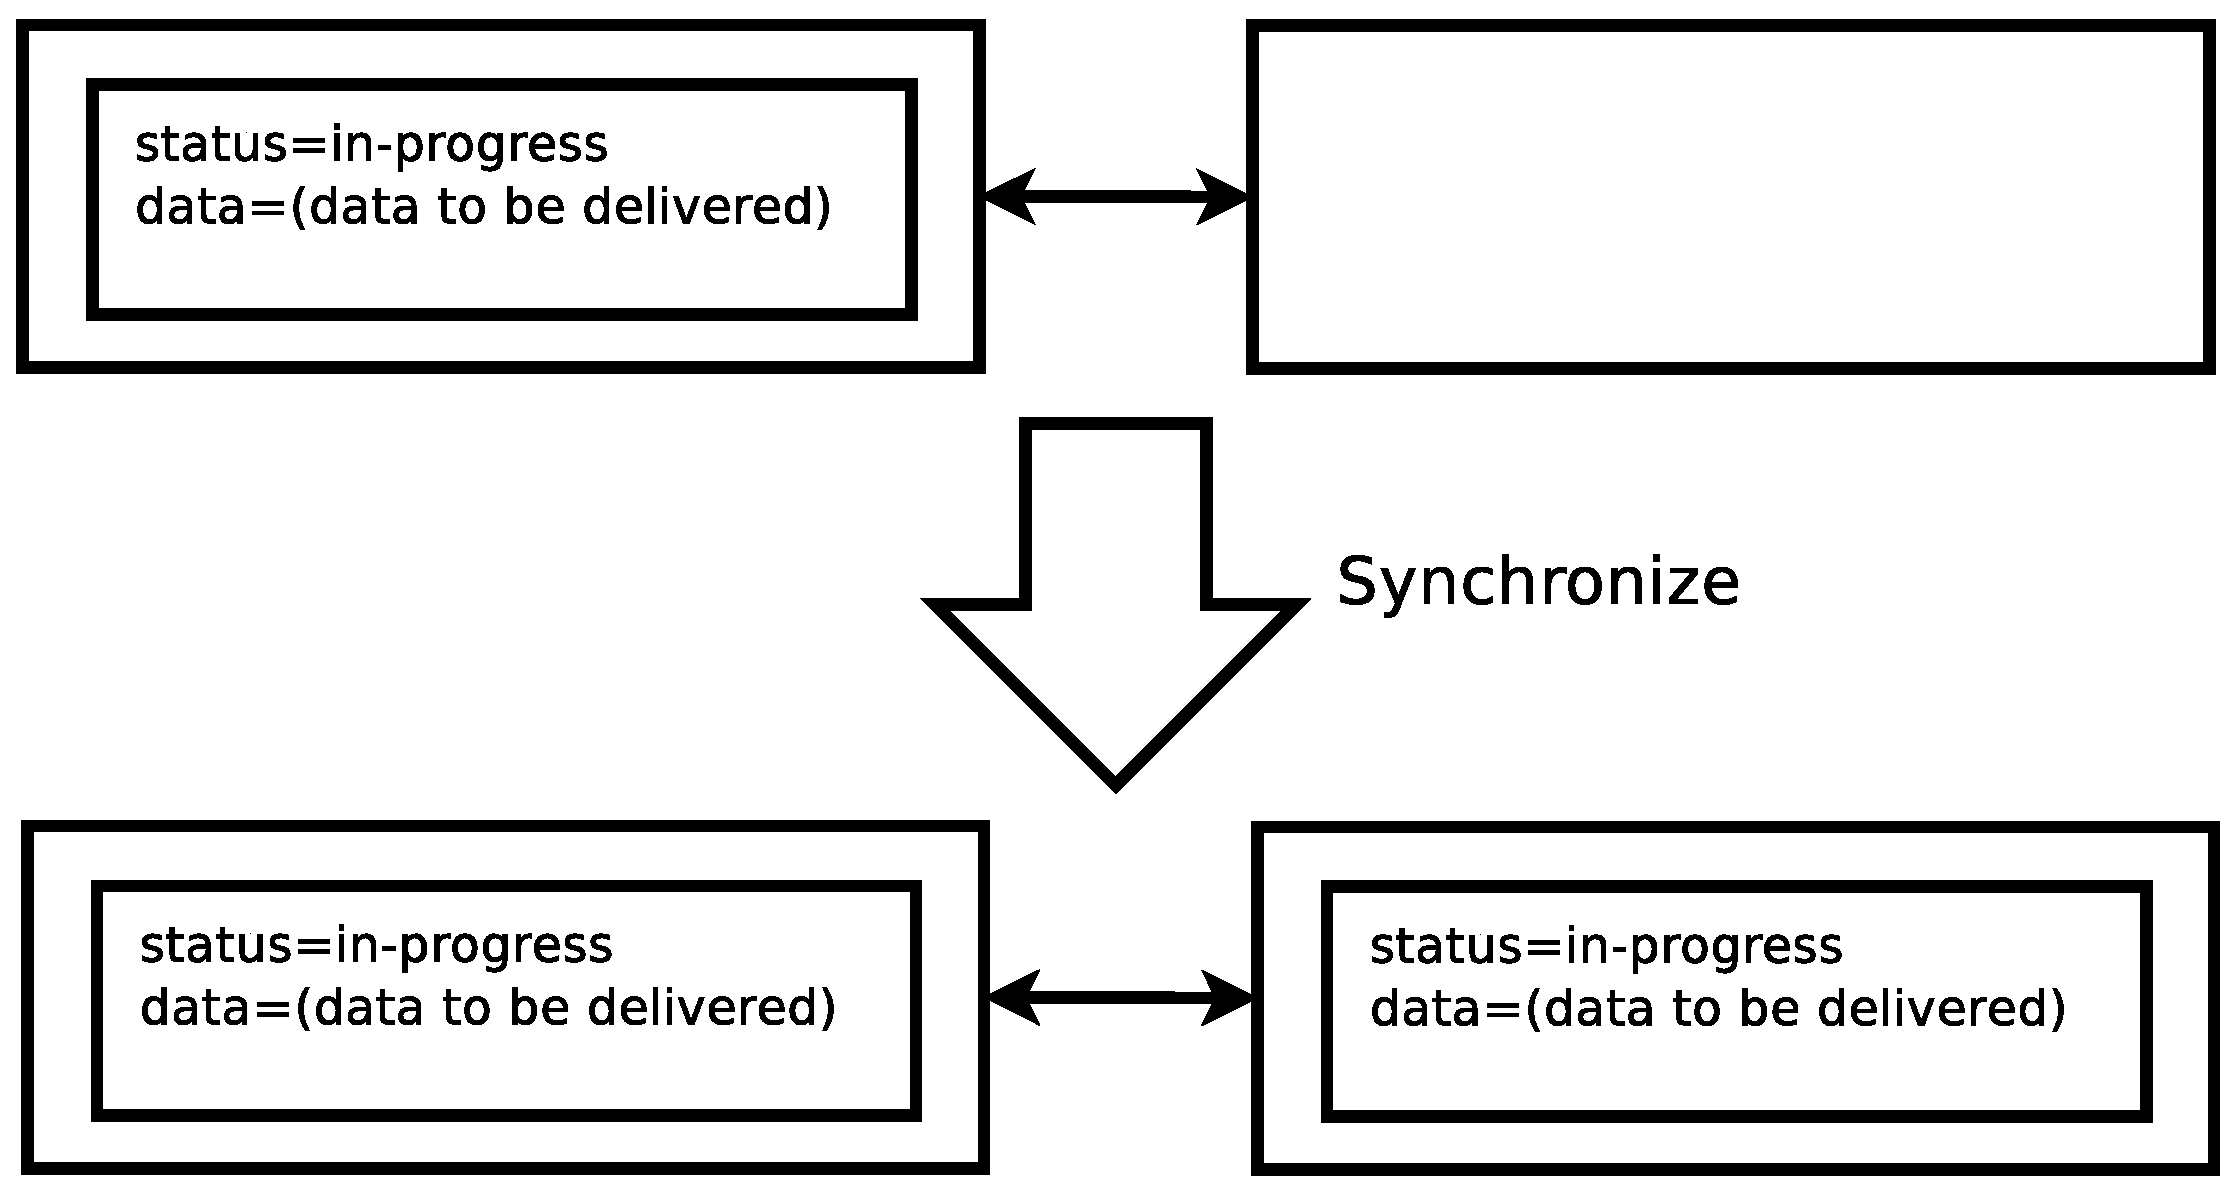
\includegraphics[width=0.3\textwidth]{rulea.eps} & 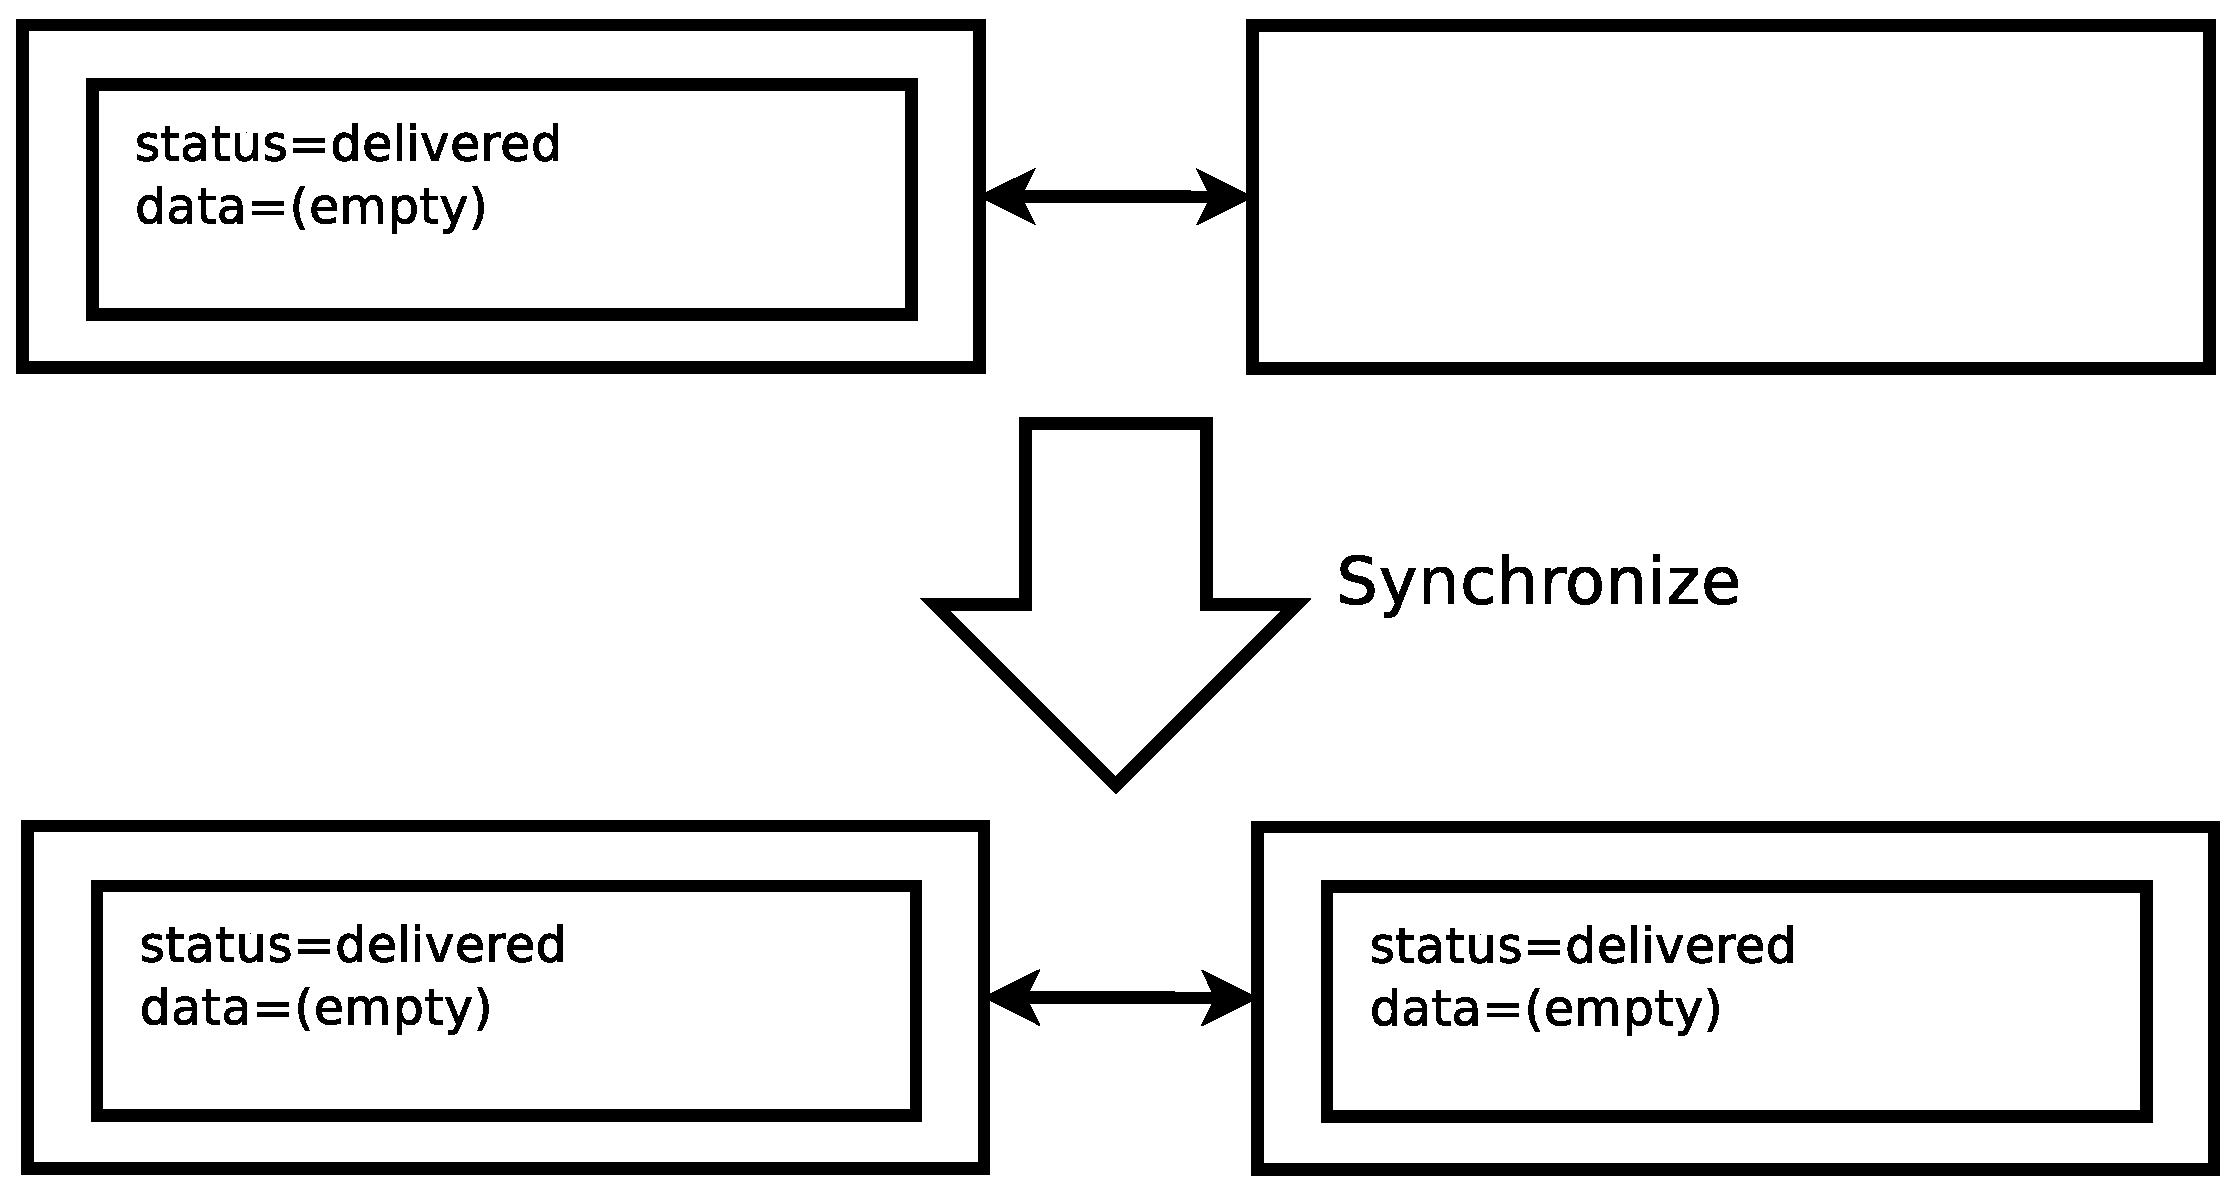
\includegraphics[width=0.3\textwidth]{ruleb.eps} & 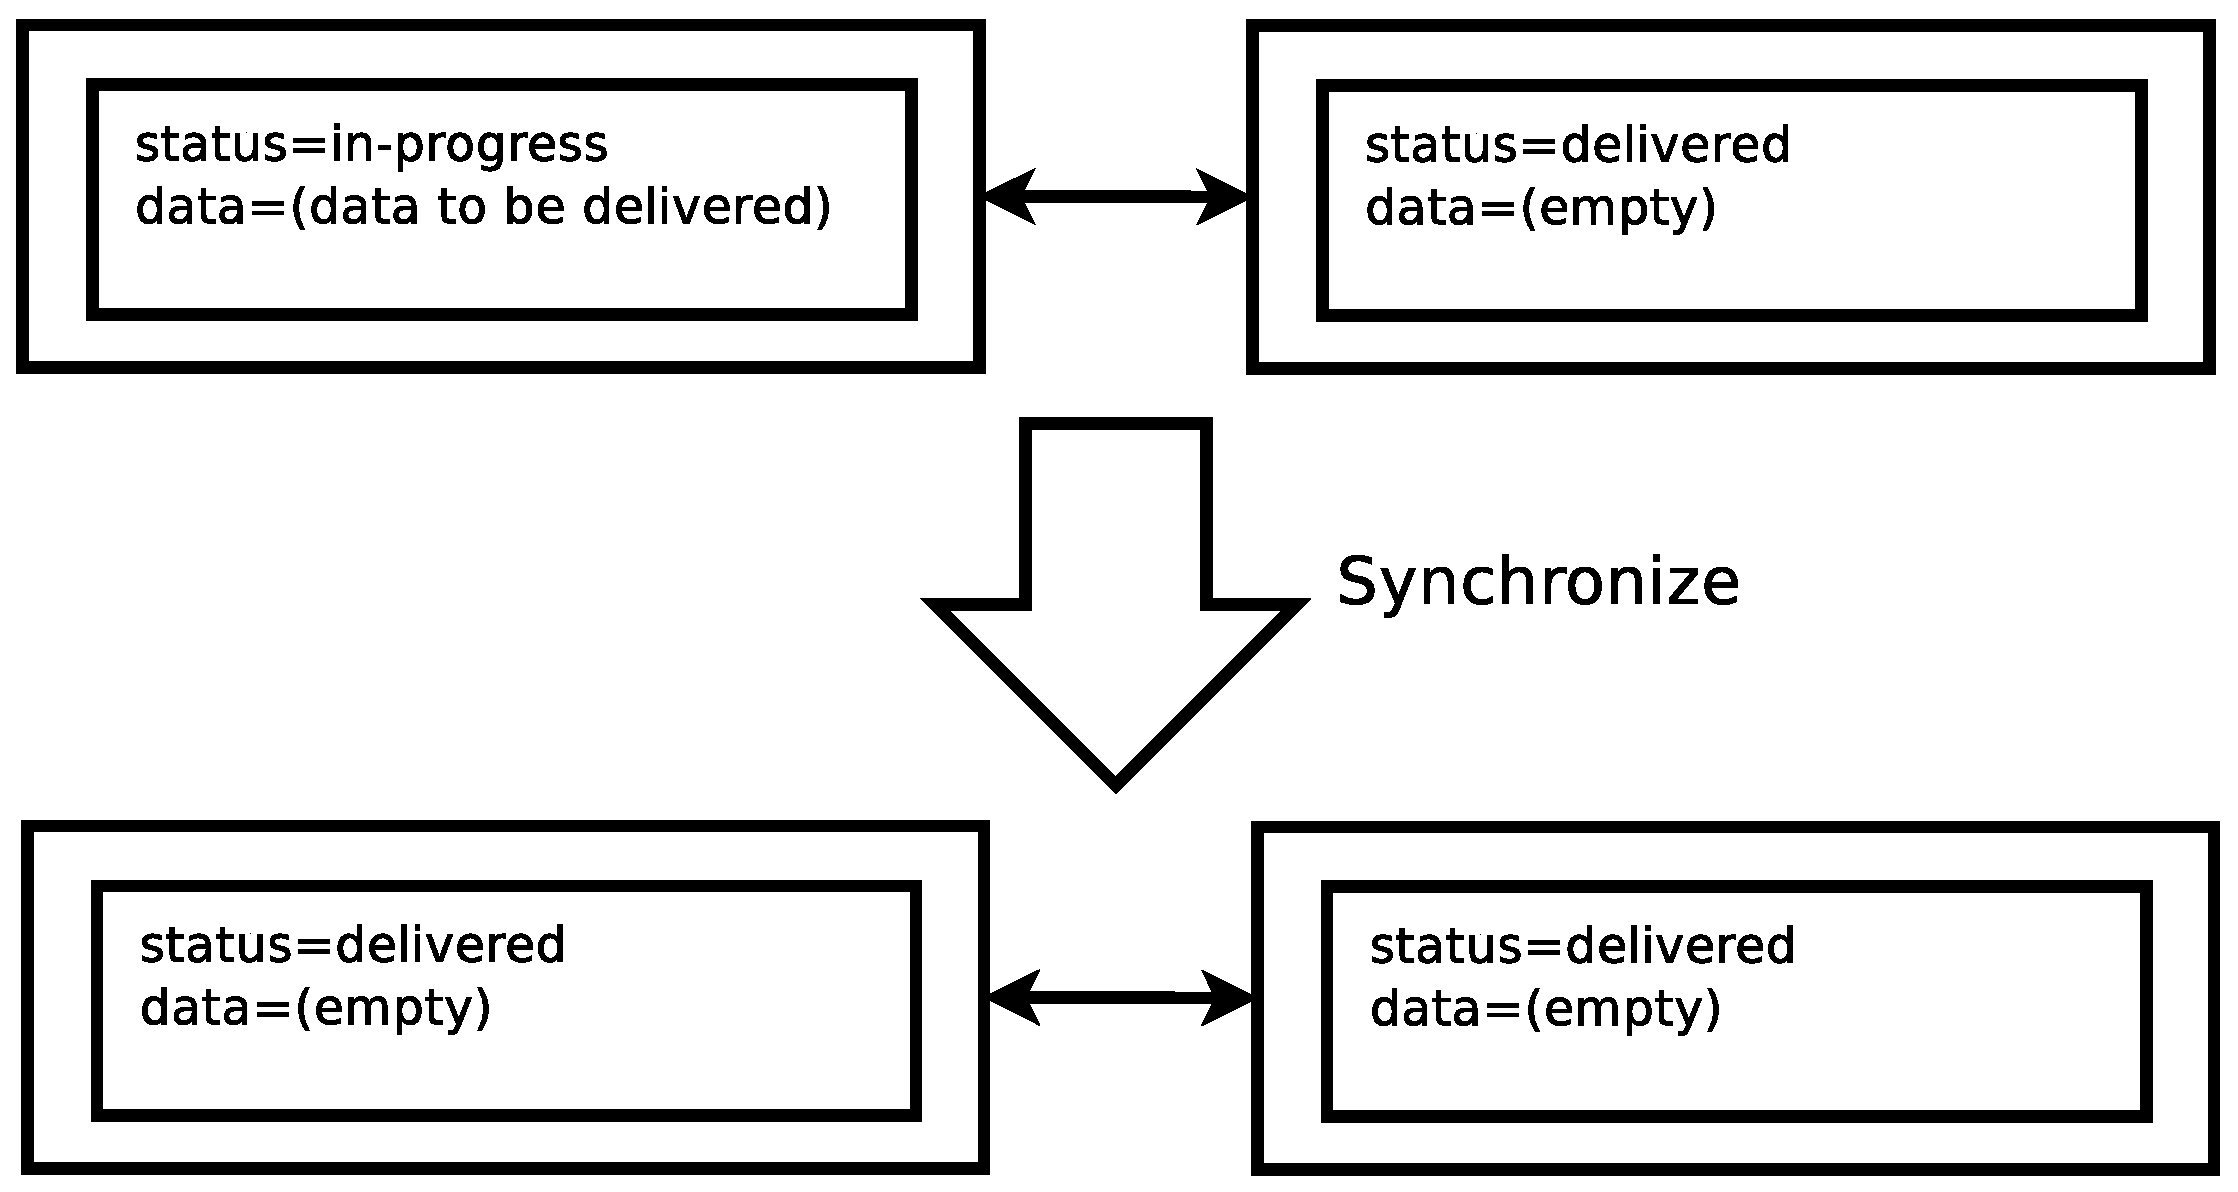
\includegraphics[width=0.3\textwidth]{rulec.eps} \\
    (a) & (b) & (c)
  \end{tabular}
  \caption{Rules for synchronizing packets.}
  \label{fig:rules}
\end{figure}

\subsection{Complete packet delivery example}
\label{sec:delivery}
Using the mechanisms previously explained, we illustrate a complete delivery from \anemobox{} to the \anemolab{} in Fig.~\ref{fig:delivery}. In (a), a packet of boat logs are just about to be delivered over bluetooth from the \anemobox{} to the \phone{}. In (b), the packet to be delivered is on the phone and about the be delivered to the \anemolab{}. There is no longer any connection to the \anemobox{}. In (c), all devices now have the same packet and it has reached the destination. From (d) to (f), the fact that the packet has been delivered is propagated backwards from the \anemolab{} to the \anemobox{}.
\begin{figure}
  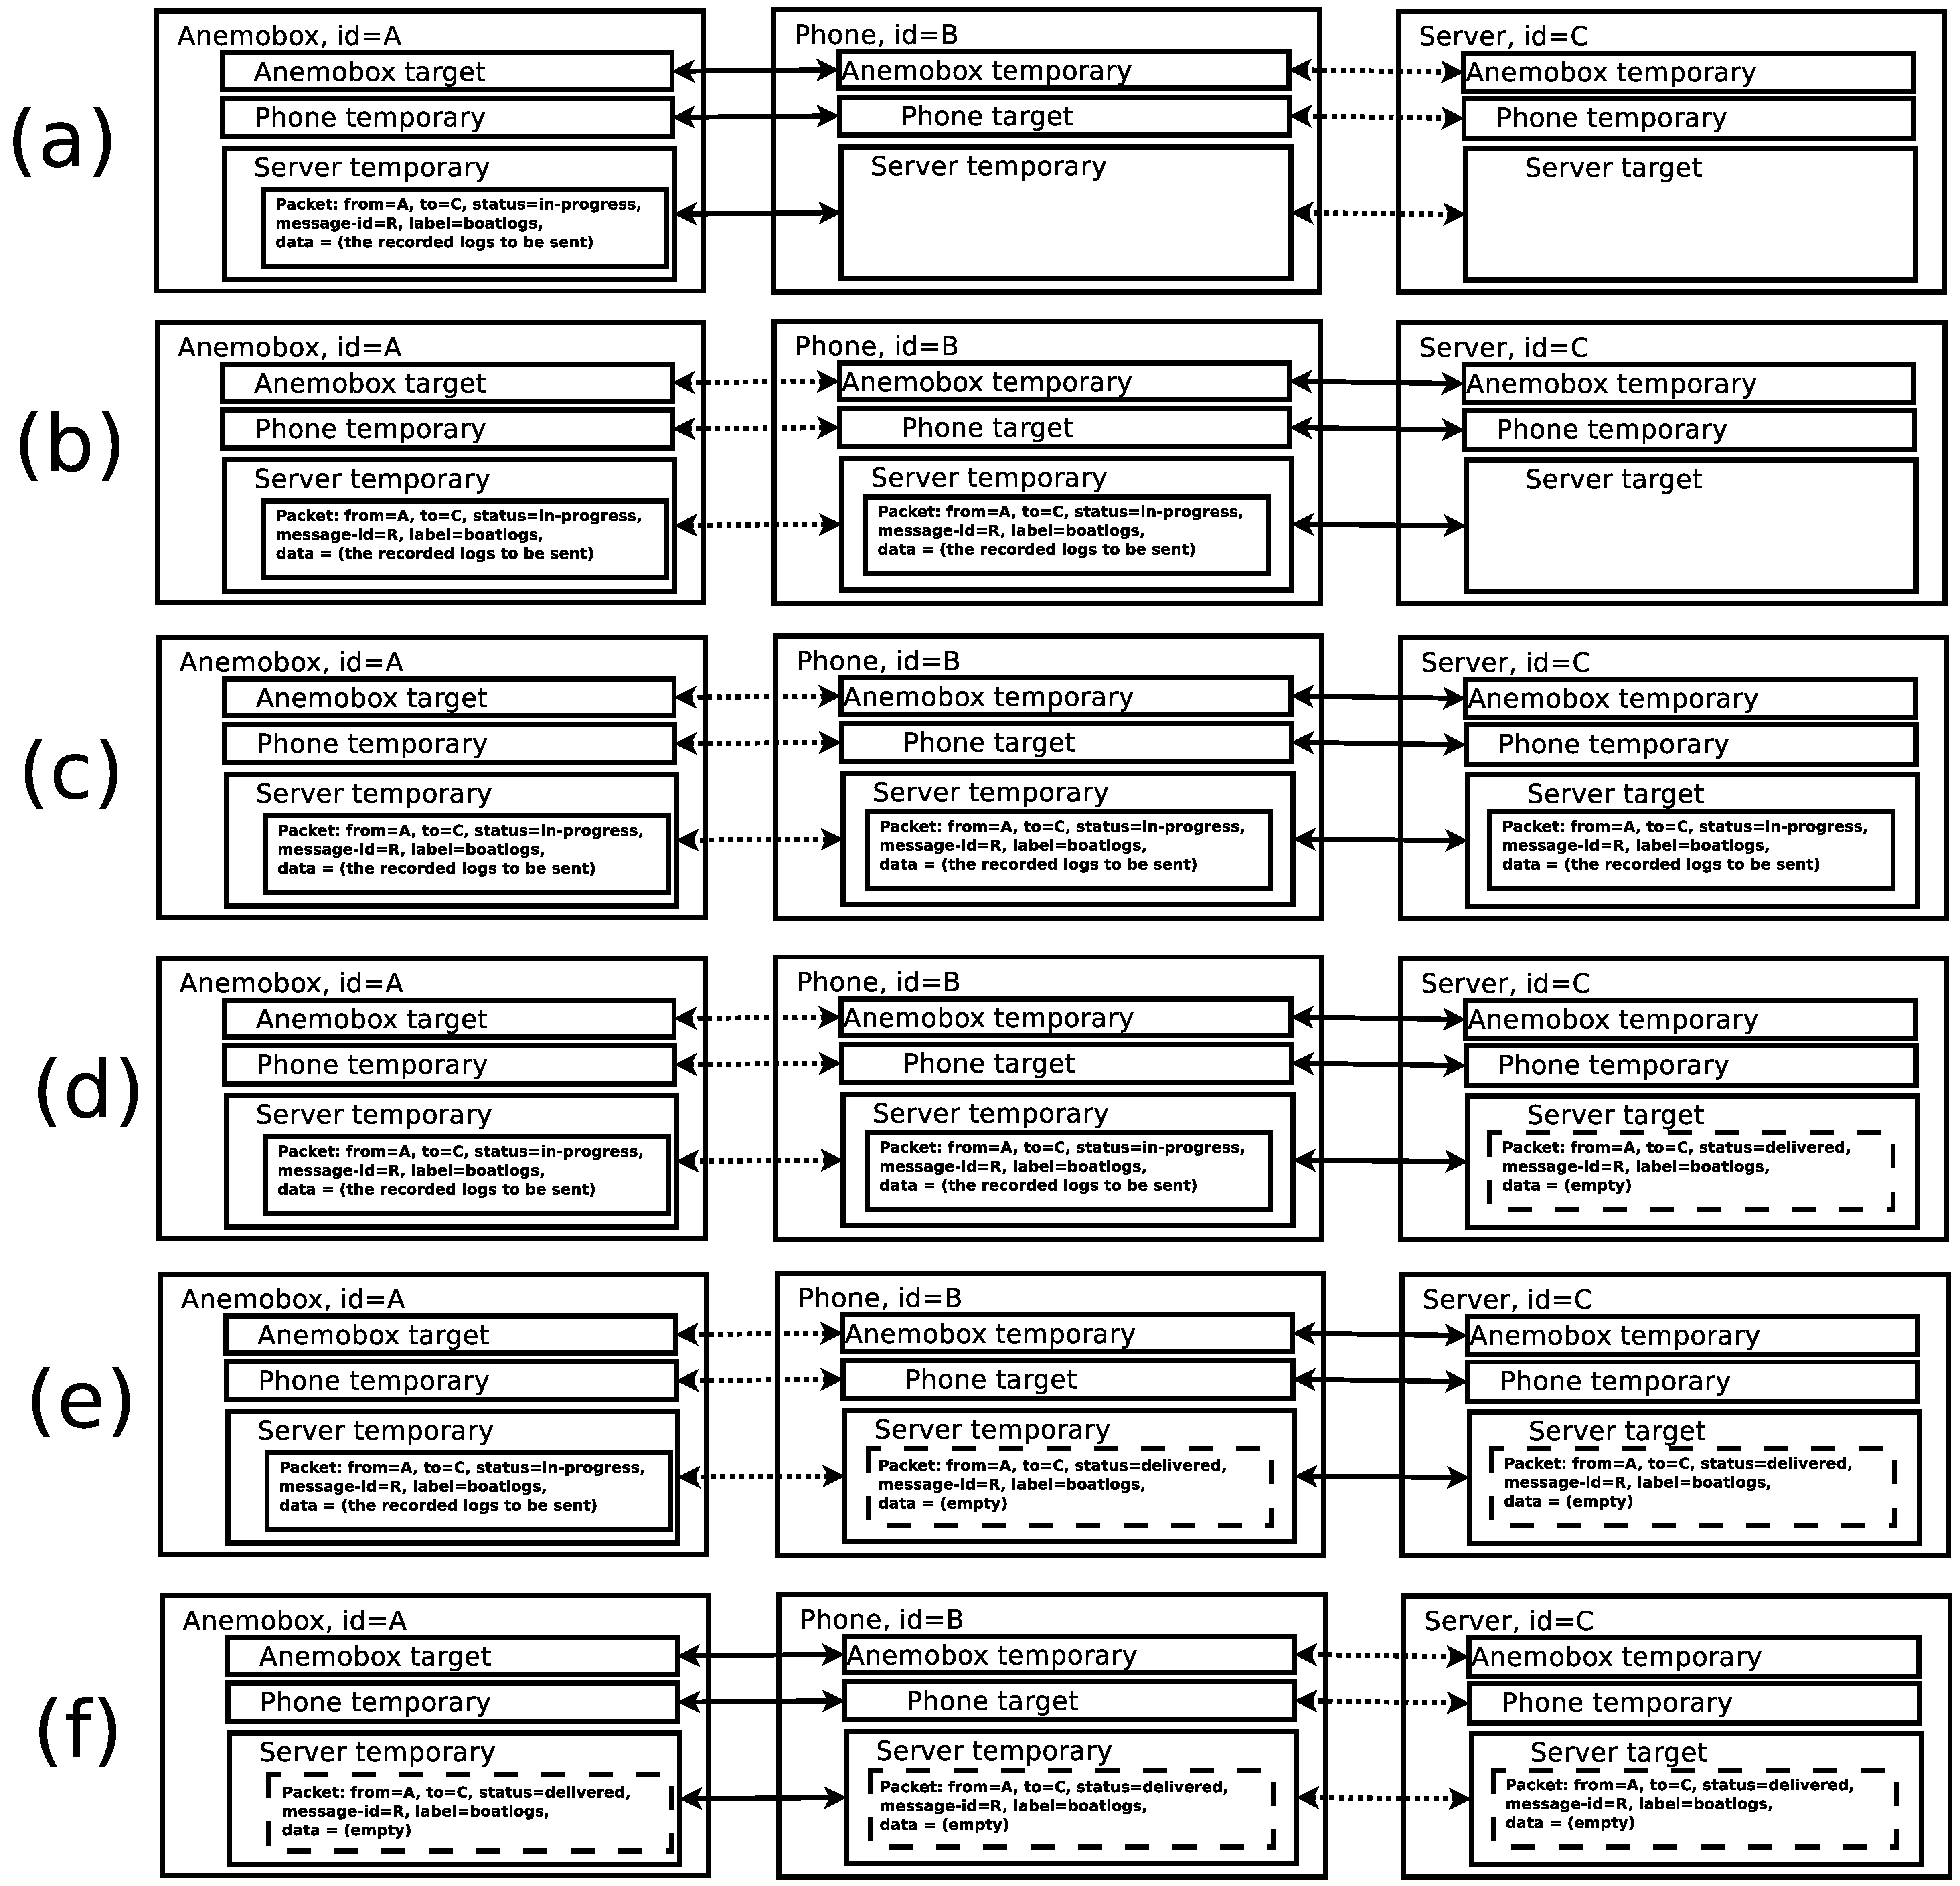
\includegraphics[width=\textwidth]{syncexample.eps}
  \caption{Delivery of boat logs from \anemobox{} to \anemolab{}.}
  \label{fig:delivery}
\end{figure}

\subsection{Garbage collection}
\label{sec:gc}
Every packet that is being sent generates some garbage that is being spread out across multiple devices. Even if the data is removed from a packet that is marked \texttt{delivered}, it is still going to consume some space on the device. The mechanism for reducing the amount of garbage is as follows: Whenever the number of packets sent from a device that are also marked \texttt{delivered} on that same device exceeds a number $n$, all those packets are removed from the device and a new packet with \texttt{label} set to \texttt{collect-garbage} is put in the temporary mailboxes of all other devices. This packet contains a list of all the packets that can be safely removed and whenever a device receives this packet, it will take action to remove all packets listed in the \texttt{data}. The packet with \texttt{label = collect-garbage} will, apart from this action, go through the same life cycle as any other packet. Even if this special garbage collection packet by itself generates some garbage through its own existence, it will result in the removal of many more packets so on the average, there will be more space available after the garbage collection packet has been propagated to all devices as long as $n$ is reasonably high.

Any device that receives the the garbage collection packet is free to decide for itself whether or not to actually remove the packets listed in the garbage collection packet.

\section{Discussion}
Some domain specific optimizations may be possible sometimes, in order to reduce the amount of data transferred and stored. For instance, if we are about to send data from the \phone{} to \anemolab{}, there is no point in propagating that data to the \anemobox{}, unless the \anemobox{} has some other connection to \anemolab{} than through the \phone{}.

We outline in a separate document the details about the protocol used for synchronizing two devices and their mailboxes. This protocol will specify how to devices talk with each other in order to synchronize.
\end{document}

